%%%%%%%%%%%%%%%%%%%%%%%%%%%%%%%%%%%%%%%%%%%%%%%%%
%%%%              APPENDIX                   %%%%
%%%%%%%%%%%%%%%%%%%%%%%%%%%%%%%%%%%%%%%%%%%%%%%%%

\newpage
\appendix
\renewcommand{\theHsection}{appendix.\Alph{section}}  % fix duplicate hyperref destinations

% ══════════════════════════════════════════════════════════════════════════════
% APPENDIX A — Sparse Retriever Hyperparameter Tuning Figures
% ══════════════════════════════════════════════════════════════════════════════
\section{Sparse Retriever Hyperparameter Tuning Figures}
\label{app:sparse_figs}

\begin{figure}[H]
  \centering
  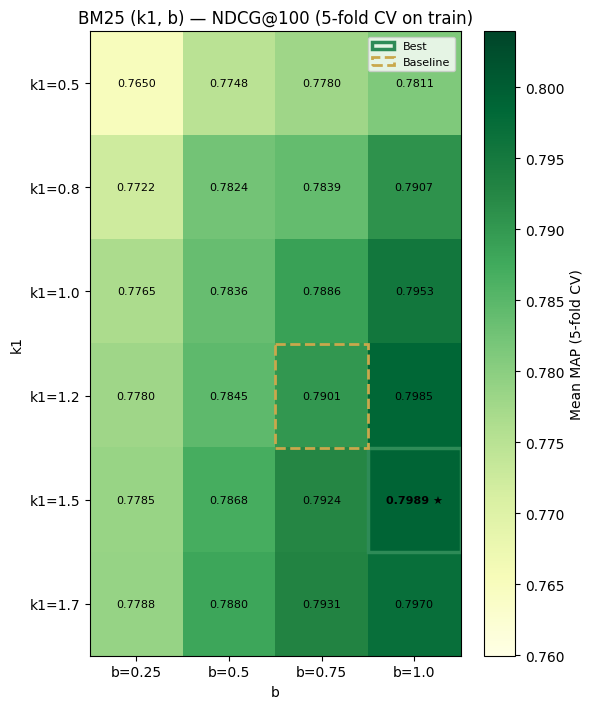
\includegraphics[width=0.70\linewidth]{images/bm25_param_sweep.png}
  \caption{BM25 $k_1$/$b$ sweep --- mean CV NDCG@100. Winner: $k_1$=1.5,
           $b$=1.0.}
  \label{fig:bm25_sweep}
\end{figure}

\begin{figure}[H]
  \centering
  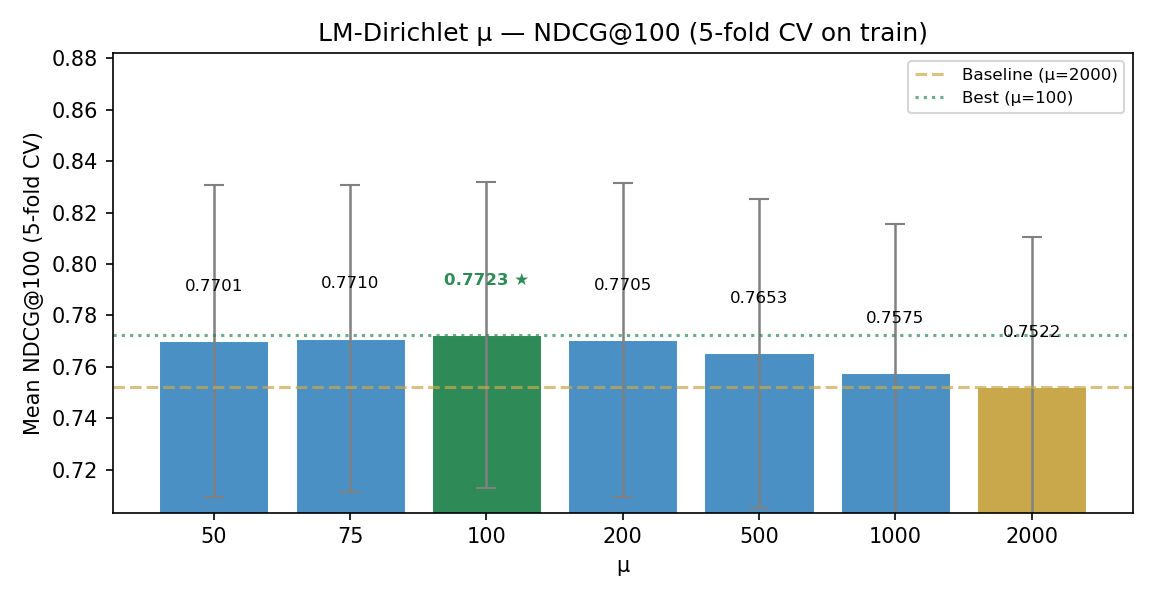
\includegraphics[width=0.92\linewidth]{images/lmdir_mu_sweep.png}
  \caption{LM-Dir $\mu$ sweep --- mean CV NDCG@100. Default $\mu$=2000
           drastically under-performs; winner is $\mu$=100.}
  \label{fig:lmdir_sweep}
\end{figure}

\begin{figure}[H]
  \centering
  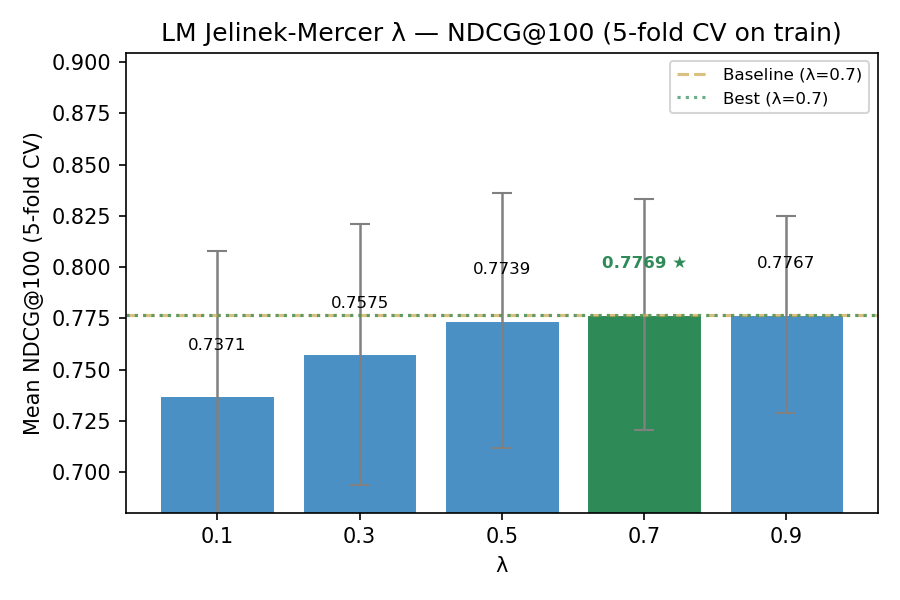
\includegraphics[width=0.82\linewidth]{images/lmjm_lambda_sweep.png}
  \caption{LM-JM $\lambda$ sweep --- NDCG@100 plateaus in the 0.65--0.75 range;
           extended grid winner $\lambda$=0.65.}
  \label{fig:lmjm_sweep}
\end{figure}

% ══════════════════════════════════════════════════════════════════════════════
% APPENDIX B — RRF Sparse+Dense Fusion Results
% ══════════════════════════════════════════════════════════════════════════════
\section{RRF Sparse+Dense Fusion Results}
\label{app:rrf_figs}

\begin{figure}[H]
  \centering
  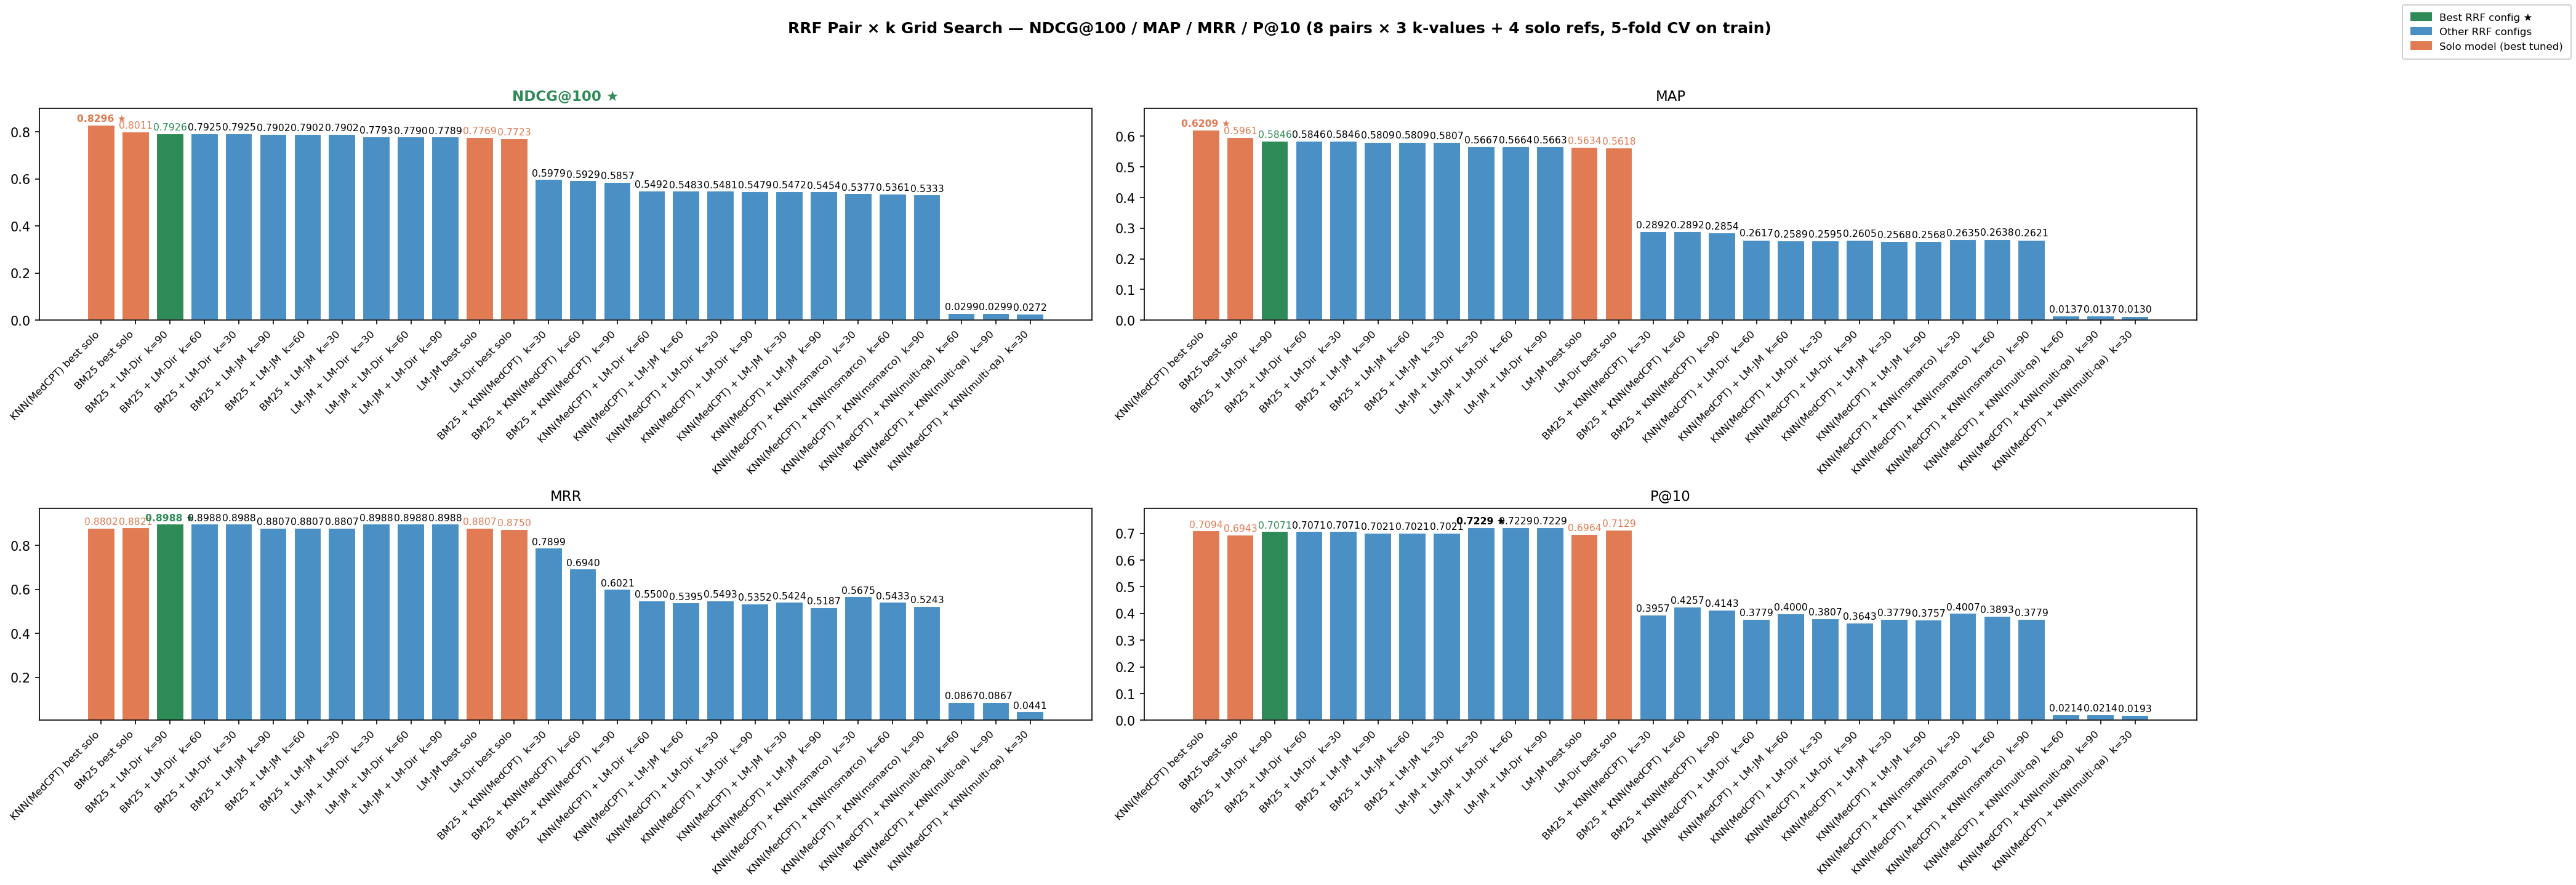
\includegraphics[width=\linewidth]{images/rrf_pair_sweep.png}
  \caption{RRF pair sweep --- 9 strategy pairs $\times$ 3 $k$ values, 5-fold CV.
           Lexical pairs (BM25+LM-Dir, $k$=90, NDCG@100=0.7907) outperform
           KNN fusions at the rank-level.}
  \label{fig:rrf_sweep}
\end{figure}

% ══════════════════════════════════════════════════════════════════════════════
% APPENDIX C — Tuning Summary
% ══════════════════════════════════════════════════════════════════════════════
\section{Tuning Summary}
\label{app:tuning_summary}

\begin{figure}[H]
  \centering
  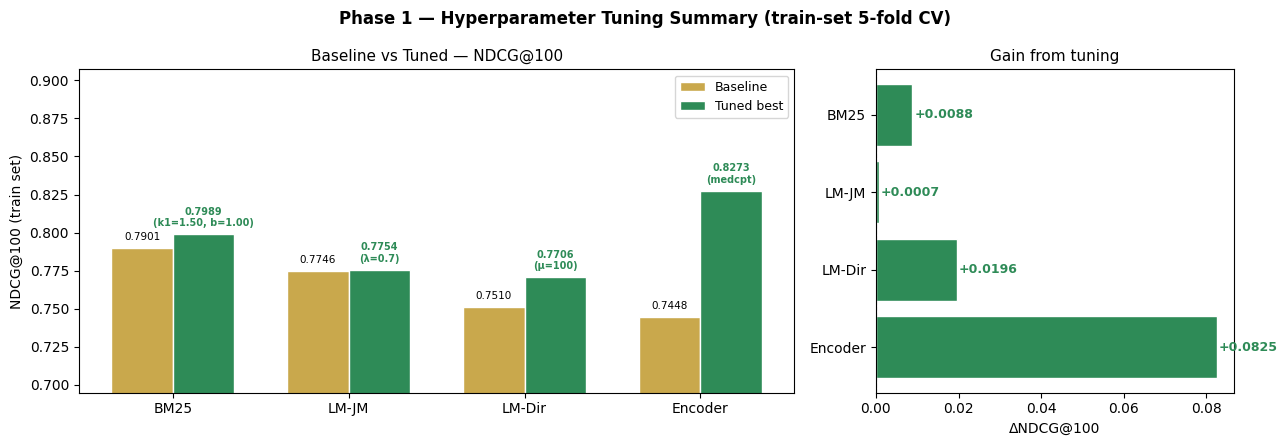
\includegraphics[width=\linewidth]{images/tuning_summary.png}
  \caption{Tuning summary: baseline vs.\ tuned NDCG@100 for every model
           (5-fold CV on 32 train topics). Encoder selection (MedCPT) yields
           the largest gain ($\Delta$NDCG@100=+0.0825 over msmarco); LM-Dir
           correction ($\mu$=100) yields the second-largest (+0.0196).}
  \label{fig:tuning_summary}
\end{figure}

\begin{figure}[H]
  \centering
  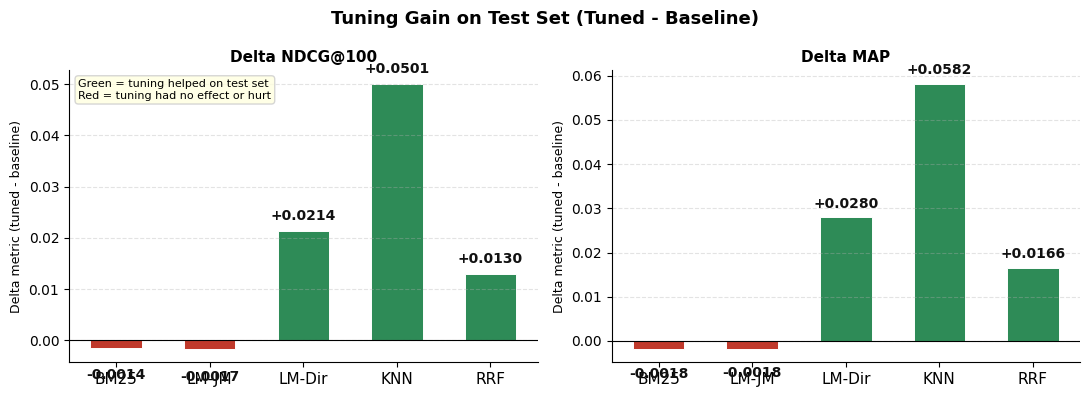
\includegraphics[width=\linewidth]{images/tuning_gain_test.png}
  \caption{Tuning gain on the test set ($\Delta$NDCG@100 and $\Delta$MAP,
           tuned $-$ baseline). KNN and RRF gain significantly; BM25 tuning
           yields no measurable gain ($\Delta$NDCG@100\,=\,$-$0.0014).}
  \label{fig:tuning_gain}
\end{figure}

\begin{table}[H]
\centering
\caption{Baseline (default parameters) vs tuned --- all 5 metrics on the
         33-query test set. NDCG@100 is the primary metric (graded qrels).
         Bold = best per column.}
\label{tab:test_results}
\begin{tabular}{lccccc}
  \hline
  \textbf{Strategy} & \textbf{NDCG@100} & \textbf{MAP} & \textbf{MRR}
                    & \textbf{P@10} & \textbf{R@100} \\
  \hline
  \multicolumn{6}{l}{\textit{Baseline (default parameters)}} \\
  BM25 ($k_1$=1.2, $b$=0.75)   & 0.7756 & 0.5695 & 0.7712 & 0.6333 & 0.8594 \\
  LM-JM ($\lambda$=0.7)         & 0.7586 & 0.5431 & 0.7848 & 0.6333 & 0.8303 \\
  LM-Dir ($\mu$=2000)           & 0.7341 & 0.5149 & 0.7740 & 0.6212 & 0.8100 \\
  KNN (msmarco)                 & 0.7576 & 0.5561 & 0.8384 & \textbf{0.6879} & 0.8933 \\
  RRF (default)                 & 0.8114 & 0.6100 & 0.8141 & 0.6667 & 0.8921 \\
  \hline
  \multicolumn{6}{l}{\textit{Tuned (locked parameters)}} \\
  BM25 ($k_1$=1.5, $b$=1.0)    & 0.7742 & 0.5677 & 0.7141 & 0.6333 & 0.8600 \\
  LM-JM ($\lambda$=0.65)        & 0.7569 & 0.5413 & 0.7864 & 0.6212 & 0.8303 \\
  LM-Dir ($\mu$=100)            & 0.7555 & 0.5428 & 0.7773 & 0.6061 & 0.8270 \\
  \textbf{KNN (MedCPT)}         & 0.8077 & 0.6143 & 0.8000 & 0.6788 & \textbf{0.8933} \\
  \textbf{RRF (BM25+MedCPT)}   & \textbf{0.8245} & \textbf{0.6266}
                                & \textbf{0.8394} & 0.6515 & \textbf{0.9142} \\
  \hline
\end{tabular}
\smallskip\par\noindent\small
KNN(MedCPT) is the \emph{train CV winner} (NDCG@100=0.8273).
RRF (BM25+MedCPT, $k$=60) achieves the highest \emph{test-set} NDCG@100=0.8245.
\end{table}

% ══════════════════════════════════════════════════════════════════════════════
% APPENDIX D — Precision-Recall Curves
% ══════════════════════════════════════════════════════════════════════════════
\section{Precision-Recall Curves}
\label{app:pr_curves}

\begin{figure}[H]
  \centering
  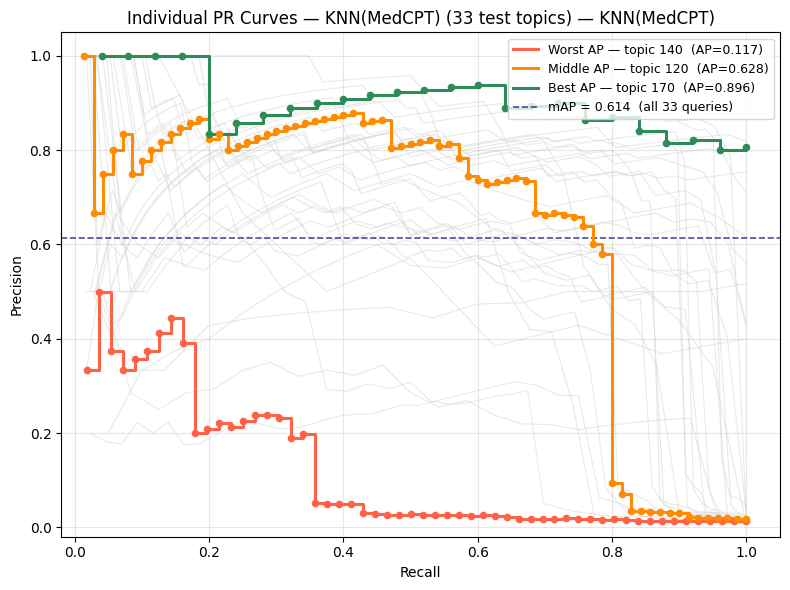
\includegraphics[width=0.85\linewidth]{images/individual_pr_curves.png}
  \caption{Per-topic PR curves for KNN(MedCPT) on all 33 test topics.
           Green = best topic (170 --- isoniazid hepatotoxicity, AP=0.8961);
           red = worst topic (140 --- spontaneous hand fractures, AP=0.1168);
           orange = median topic (120 --- causes of facial numbness, AP=0.6277).
           Gray curves = remaining 30 topics.
           Dashed navy = mean AP (MAP=0.6143).}
  \label{fig:individual_pr}
\end{figure}

\begin{figure}[H]
  \centering
  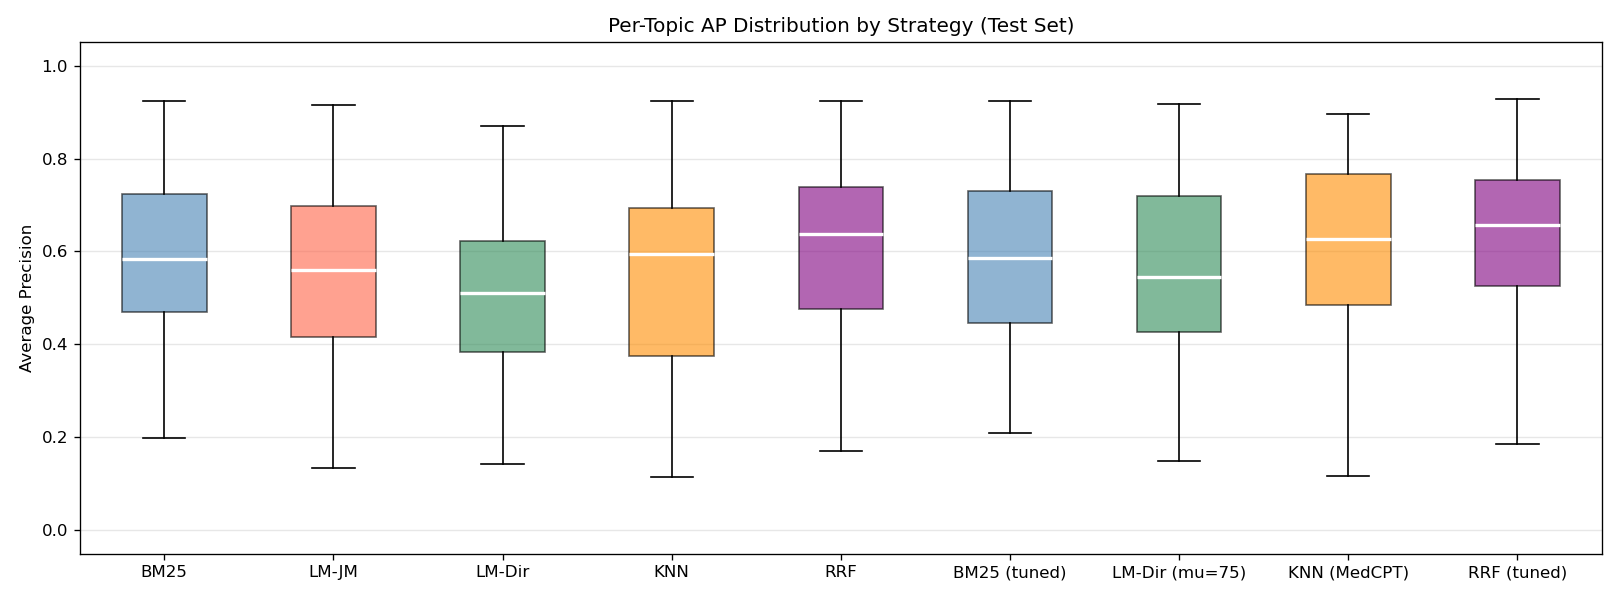
\includegraphics[width=0.80\linewidth]{images/ap_boxplot.png}
  \caption{Per-topic AP distribution across all strategies (test set, 33
           topics). RRF (tuned) achieves the highest median AP and the least
           variance. Wide IQR reflects inherent topic-difficulty spread.}
  \label{fig:ap_boxplot}
\end{figure}

% ══════════════════════════════════════════════════════════════════════════════
% APPENDIX E — Phase 2 Images
% ══════════════════════════════════════════════════════════════════════════════

\begin{figure}[H]
  \centering
  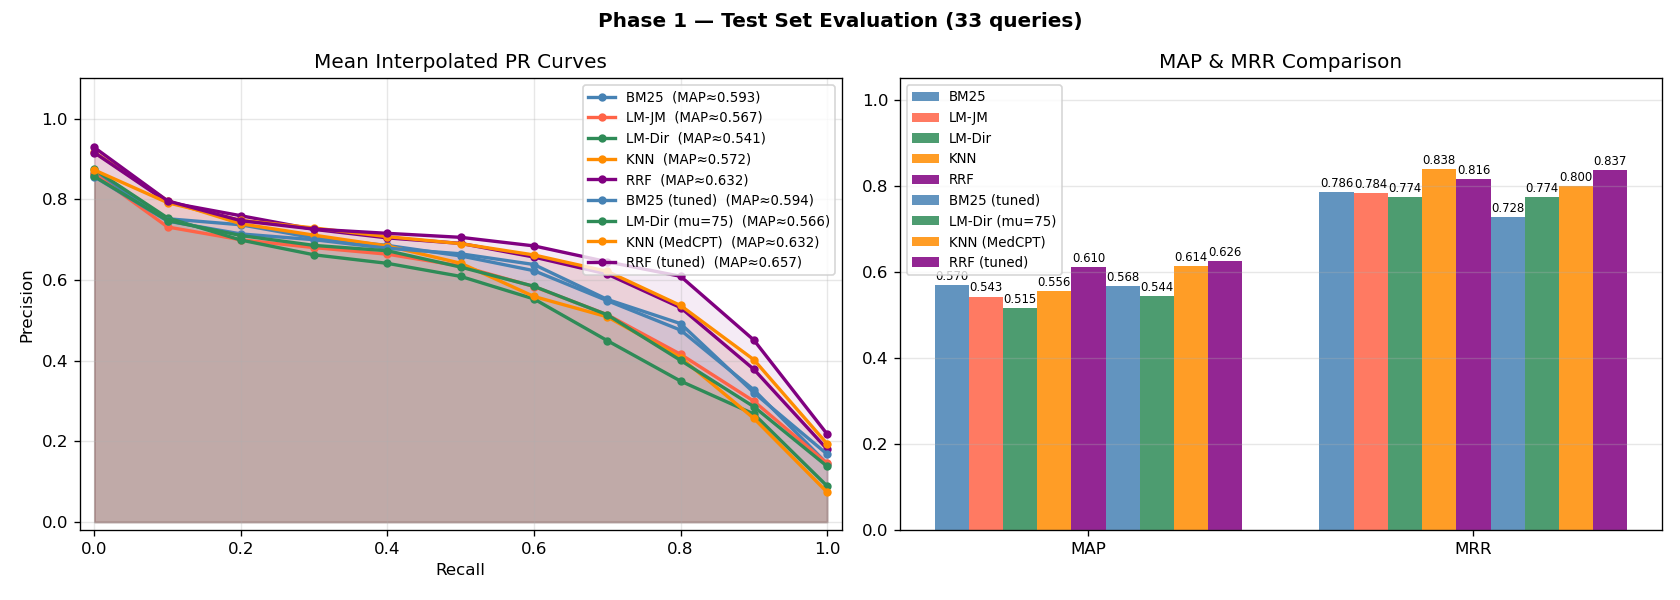
\includegraphics[width=\linewidth]{images/pr_curves.png}
  \caption{Mean interpolated PR curves for all strategies on the 33-query
           test set (left) with MAP/MRR bar chart (right). RRF (tuned) and
           KNN (MedCPT) dominate across the full recall range.}
  \label{fig:pr_curves}
\end{figure}

\begin{figure}[H]
  \centering
  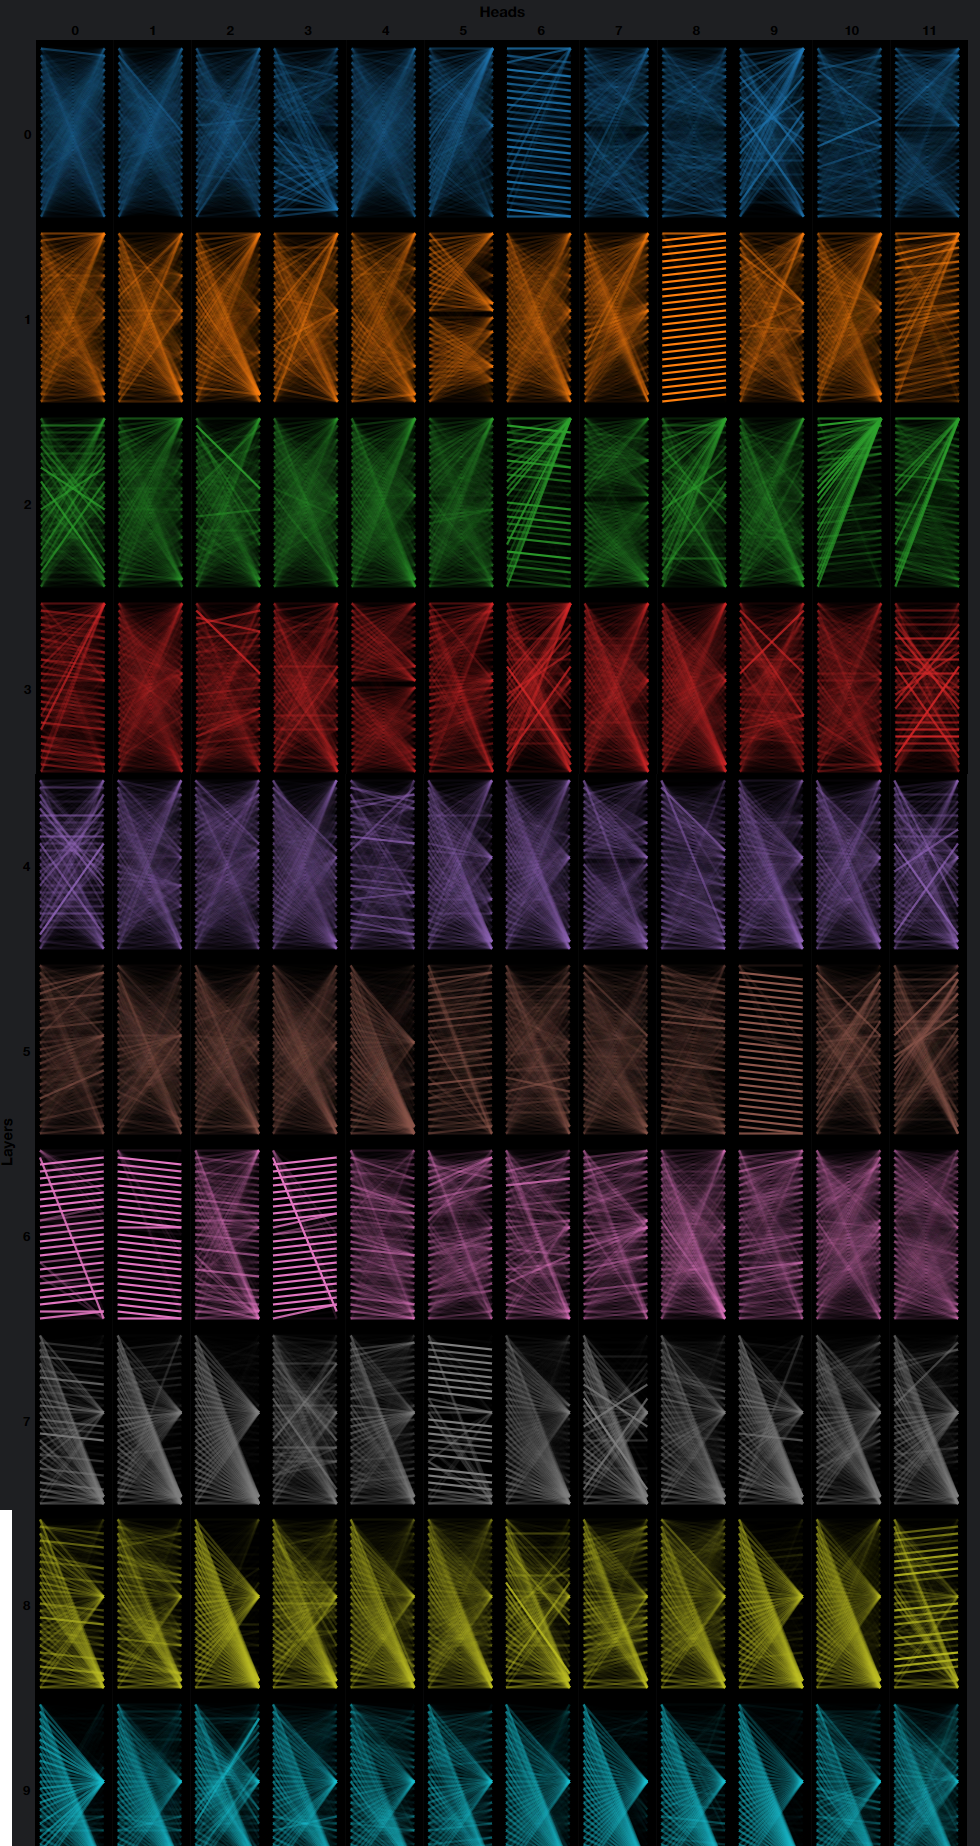
\includegraphics[width=\linewidth]{images/model_view.png}
  \caption{(Nearly) all layers' multi-head self-attentions visualization}
  \label{fig:model_view}
\end{figure}

\begin{figure}[H]
  \centering
  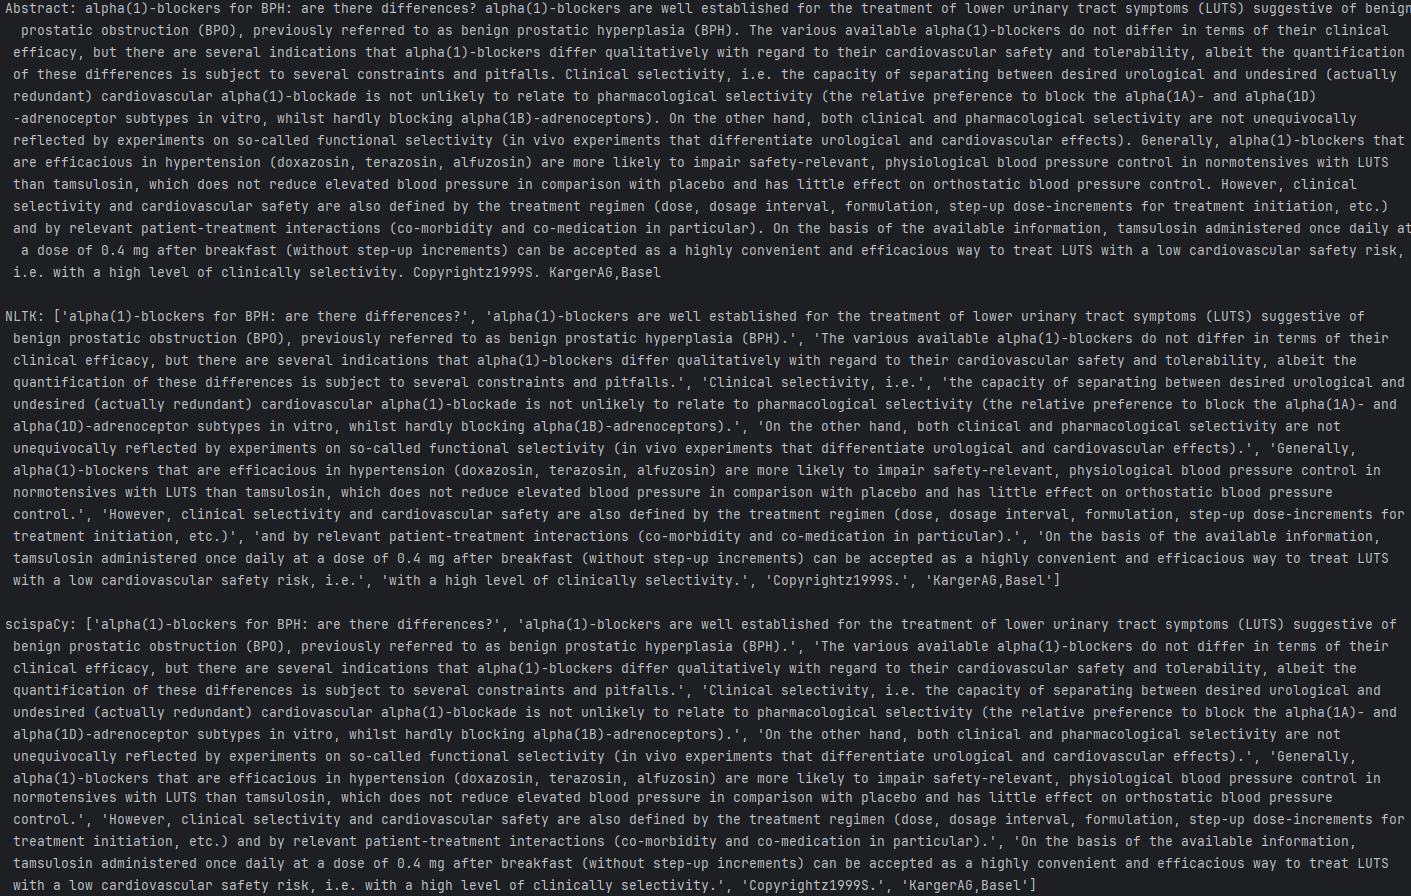
\includegraphics[width=\linewidth]{images/nltk_sciscpacy_ex2.png}
  \caption{Additional NLTK vs. scispaCy example}
  \label{fig:nltk_sciscpacy_ex2}
\end{figure}

\begin{figure}[H]
  \centering
  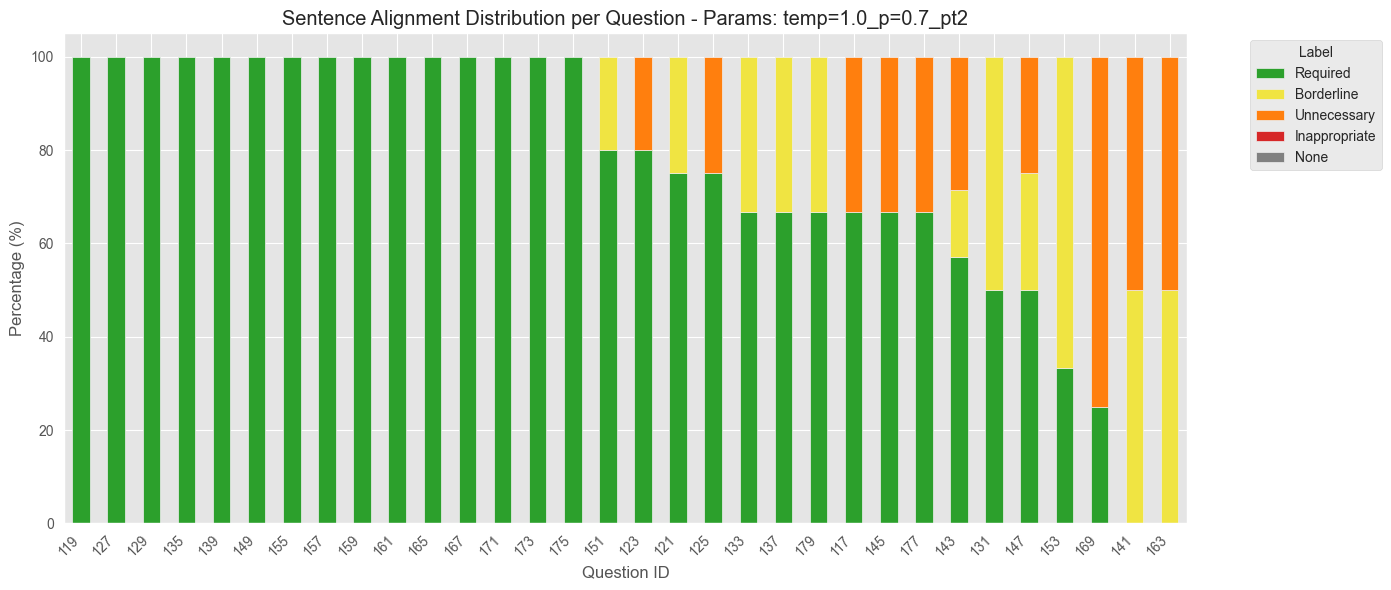
\includegraphics[width=\linewidth]{images/full_sentence_segmentation_best_unlimited.png}
  \caption{Sentence segmentation results for all queries for best unlimited model}
  \label{fig:full_sentence_segmentation_best_unlimited}
\end{figure}

\begin{figure}[H]
  \centering
  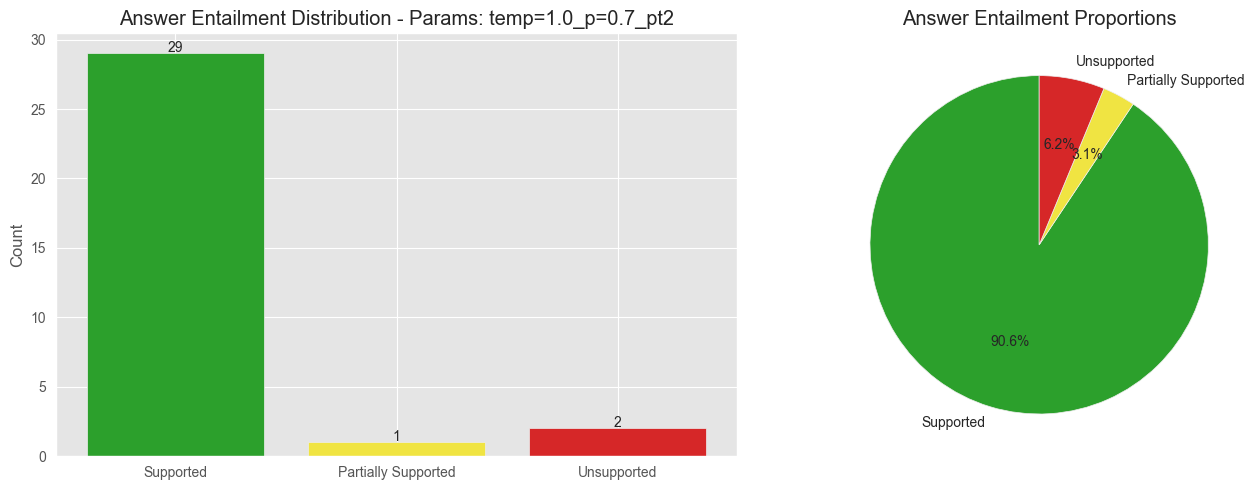
\includegraphics[width=\linewidth]{images/full_answer_entailment_best_unlimited.png}
  \caption{Answer entailment results for all queries for best unlimited model}
  \label{fig:full_answer_entailment_best_unlimited}
\end{figure}

\begin{table}[htbp]
\centering
\caption{Gemma 4 31B IT Testing Parameters}
\label{tab:gemma_parameters}
\begin{tabular}{cccc}
  \hline
  \textbf{Property} & \textbf{Values} \\
  \hline
  Temperature & [0.0, 0.3, 0.7, 1.0] \\
  Top-p & [1.0, 0.9, 0.7] \\
  Prompt & [Context \& Topic \& Question \& Narrative, Context \& Question] \\
  Max sentences per doc & [3, unlimited] \\
  \hline
\end{tabular}
\end{table}